\section{Variantes da LCS}

\begin{frame}[fragile]{Identificação da LCS}

    \begin{itemize}
        \item Assim como o problema de \textit{edit distance}, uma variante comum do LCS é
            determinar a sequência de operações que leva à maior subsequência comum

        \item A implementação é idêntica à proposta para $edit(S, T)$, uma vez aplicada a 
            modificação dos pesos e a alteração da operação \code{cpp}{min()} por 
            \code{cpp}{max()}, de modo que a complexidade permanece sendo $O(nm)$

        \item A maior subsequência comum corresponde aos caracteres onde os caracteres foram
            mantidos

        \item Assim esta rotina pode ser modificada para exibir a sequência, e não as operações
            que levaram a ela
    \end{itemize}

\end{frame}

\begin{frame}[fragile]{Identificação da LCS em C++}
    \inputsnippet{cpp}{74}{93}{codes/lcs2.cpp}
\end{frame}

\begin{frame}[fragile]{Identificação da LCS em C++}
    \inputsnippet{cpp}{95}{114}{codes/lcs2.cpp}
\end{frame}

\begin{frame}[fragile]{Identificação da LCS em C++}
    \inputsnippet{cpp}{116}{124}{codes/lcs2.cpp}
\end{frame}

\begin{frame}[fragile]{LCS e LIS}

    \begin{itemize}
        \item Quando todos os caracteres de $S$ e de $T$ são distintos (isto é, 
            $S[i] \neq S[j]$ se $i \neq j$, o mesmo para $T$), o problema de se determinar a LCS 
            pode ser reduzido ao problema de se determinar a maior sequência crescente 
            (\textit{Longest Increasing Subsequence -- LIS})

        \item Para tal, seja $\lbrace a_i\rbrace$ a sequência crescente de índices de $S$ tais que
            $S[a_i] = T[j]$ para algum $j\in [1,m]$

        \item Em outras palavras, $\lbrace a_i\rbrace$ é sequência crescente de índices de 
            caracteres de $S$ que coincidem com algum dos caracteres de $T$

        \item Seja $\lbrace b_k\rbrace$ a sequência tal que $b_k = j_k$, onde $S[a_k] = T[j_k$] 

        \item A LIS de $\lbrace b_k\rbrace$ corresponderá a LCS entre as duas strings

        \item A vantagem desta abordagem é que, enquanto a LCS tem implementação $O(nm)$, a LIS 
            pode ser implementada em $O(n \log n)$

    \end{itemize}

\end{frame}

\begin{frame}[fragile]{Visualização do algoritmo linearítmico para a LIS}

    \begin{figure}[h]
        \centering
        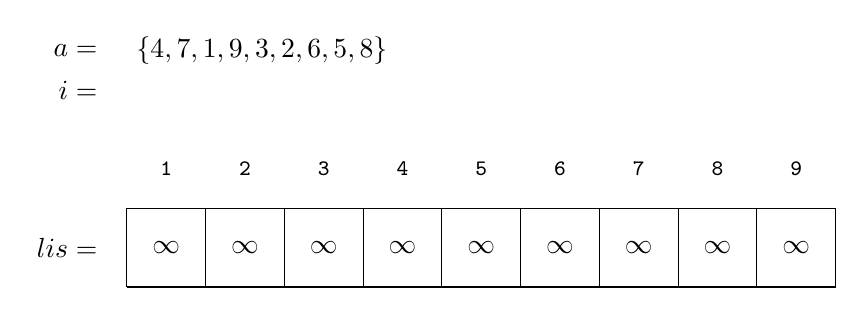
\begin{tikzpicture}

        \node[anchor=east] at (0.75, 4) { $a = $ };
        \node[anchor=west] at (1, 4) { $\{ 4, 7, 1, 9, 3, 2, 6, 5, 8 \}$ };
        \node[anchor=east] at (0.75, 3.5) { $i = $ };

        \node[anchor=east] at (0.75, 1.5) { $lis = $ };
        \draw (1, 1) grid (10, 2);

        \foreach \x in {1, ..., 9}
            \node at (\x + 0.5, 2.5) { \footnotesize \textbf{\texttt{\x}} };

        \node at (1.5, 1.5) { $\infty$ };
        \node at (2.5, 1.5) { $\infty$ };
        \node at (3.5, 1.5) { $\infty$ };
        \node at (4.5, 1.5) { $\infty$ };
        \node at (5.5, 1.5) { $\infty$ };
        \node at (6.5, 1.5) { $\infty$ };
        \node at (7.5, 1.5) { $\infty$ };
        \node at (8.5, 1.5) { $\infty$ };
        \node at (9.5, 1.5) { $\infty$ };
 
        \end{tikzpicture}
    \end{figure}

\end{frame}

\begin{frame}[fragile]{Visualização do algoritmo linearítmico para a LIS}

    \begin{figure}[h]
        \centering
        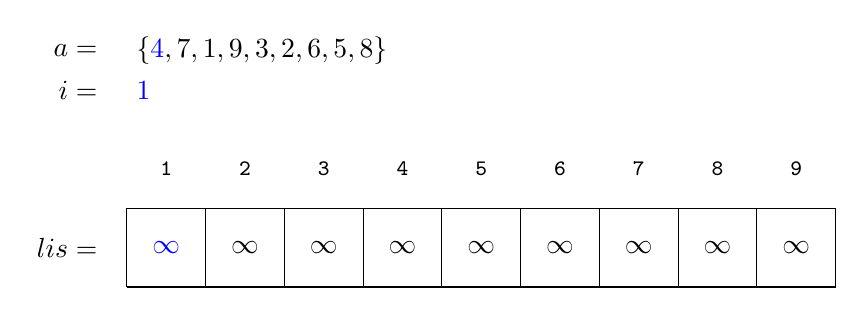
\begin{tikzpicture}

        \node[anchor=east] at (0.75, 4) { $a = $ };
        \node[anchor=west] at (1, 4) { $\{ \textcolor{blue}{4}, 7, 1, 9, 3, 2, 6, 5, 8 \}$ };
        \node[anchor=east] at (0.75, 3.5) { $i = $ };
        \node[anchor=west] at (1, 3.5) { $\textcolor{blue}{1}$ };

        \node[anchor=east] at (0.75, 1.5) { $lis = $ };
        \draw (1, 1) grid (10, 2);

        \foreach \x in {1, ..., 9}
            \node at (\x + 0.5, 2.5) { \footnotesize \textbf{\texttt{\x}} };

        \node at (1.5, 1.5) { \textcolor{blue}{$\infty$} };
        \node at (2.5, 1.5) { $\infty$ };
        \node at (3.5, 1.5) { $\infty$ };
        \node at (4.5, 1.5) { $\infty$ };
        \node at (5.5, 1.5) { $\infty$ };
        \node at (6.5, 1.5) { $\infty$ };
        \node at (7.5, 1.5) { $\infty$ };
        \node at (8.5, 1.5) { $\infty$ };
        \node at (9.5, 1.5) { $\infty$ };
 
        \end{tikzpicture}
    \end{figure}

\end{frame}

\begin{frame}[fragile]{Visualização do algoritmo linearítmico para a LIS}

    \begin{figure}[h]
        \centering
        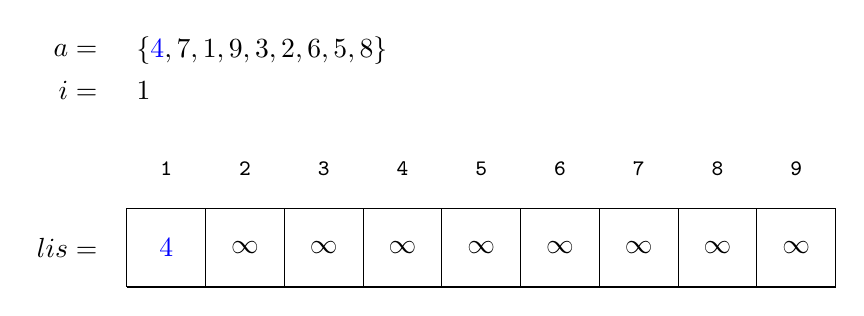
\begin{tikzpicture}

        \node[anchor=east] at (0.75, 4) { $a = $ };
        \node[anchor=west] at (1, 4) { $\{ \textcolor{blue}{4}, 7, 1, 9, 3, 2, 6, 5, 8 \}$ };
        \node[anchor=east] at (0.75, 3.5) { $i = $ };
        \node[anchor=west] at (1, 3.5) { $\textcolor{black}{1}$ };

        \node[anchor=east] at (0.75, 1.5) { $lis = $ };
        \draw (1, 1) grid (10, 2);

        \foreach \x in {1, ..., 9}
            \node at (\x + 0.5, 2.5) { \footnotesize \textbf{\texttt{\x}} };

        \node at (1.5, 1.5) { \textcolor{blue}{$4$} };
        \node at (2.5, 1.5) { $\infty$ };
        \node at (3.5, 1.5) { $\infty$ };
        \node at (4.5, 1.5) { $\infty$ };
        \node at (5.5, 1.5) { $\infty$ };
        \node at (6.5, 1.5) { $\infty$ };
        \node at (7.5, 1.5) { $\infty$ };
        \node at (8.5, 1.5) { $\infty$ };
        \node at (9.5, 1.5) { $\infty$ };
 
        \end{tikzpicture}
    \end{figure}

\end{frame}

\begin{frame}[fragile]{Visualização do algoritmo linearítmico para a LIS}

    \begin{figure}[h]
        \centering
        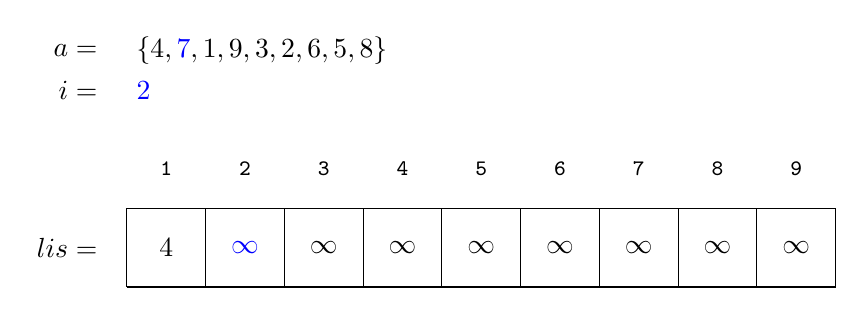
\begin{tikzpicture}

        \node[anchor=east] at (0.75, 4) { $a = $ };
        \node[anchor=west] at (1, 4) { $\{ \textcolor{black}{4}, \textcolor{blue}{7}, 1, 9, 3, 2, 6, 5, 8 \}$ };
        \node[anchor=east] at (0.75, 3.5) { $i = $ };
        \node[anchor=west] at (1, 3.5) { $\textcolor{blue}{2}$ };

        \node[anchor=east] at (0.75, 1.5) { $lis = $ };
        \draw (1, 1) grid (10, 2);

        \foreach \x in {1, ..., 9}
            \node at (\x + 0.5, 2.5) { \footnotesize \textbf{\texttt{\x}} };

        \node at (1.5, 1.5) { \textcolor{black}{$4$} };
        \node at (2.5, 1.5) { \textcolor{blue}{$\infty$} };
        \node at (3.5, 1.5) { $\infty$ };
        \node at (4.5, 1.5) { $\infty$ };
        \node at (5.5, 1.5) { $\infty$ };
        \node at (6.5, 1.5) { $\infty$ };
        \node at (7.5, 1.5) { $\infty$ };
        \node at (8.5, 1.5) { $\infty$ };
        \node at (9.5, 1.5) { $\infty$ };
 
        \end{tikzpicture}
    \end{figure}

\end{frame}

\begin{frame}[fragile]{Visualização do algoritmo linearítmico para a LIS}

    \begin{figure}[h]
        \centering
        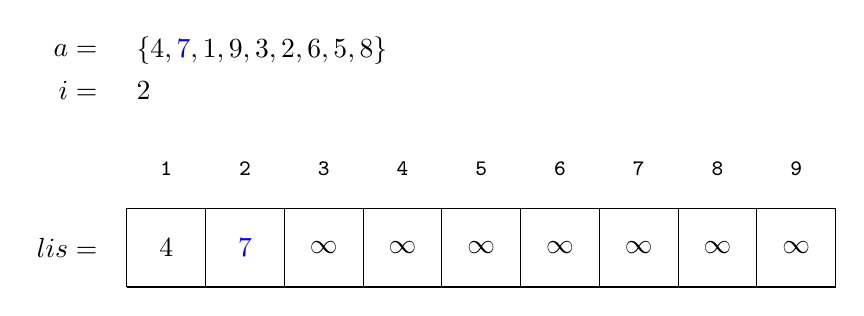
\begin{tikzpicture}

        \node[anchor=east] at (0.75, 4) { $a = $ };
        \node[anchor=west] at (1, 4) { $\{ \textcolor{black}{4}, \textcolor{blue}{7}, 1, 9, 3, 2, 6, 5, 8 \}$ };
        \node[anchor=east] at (0.75, 3.5) { $i = $ };
        \node[anchor=west] at (1, 3.5) { $\textcolor{black}{2}$ };

        \node[anchor=east] at (0.75, 1.5) { $lis = $ };
        \draw (1, 1) grid (10, 2);

        \foreach \x in {1, ..., 9}
            \node at (\x + 0.5, 2.5) { \footnotesize \textbf{\texttt{\x}} };

        \node at (1.5, 1.5) { \textcolor{black}{$4$} };
        \node at (2.5, 1.5) { \textcolor{blue}{$7$} };
        \node at (3.5, 1.5) { $\infty$ };
        \node at (4.5, 1.5) { $\infty$ };
        \node at (5.5, 1.5) { $\infty$ };
        \node at (6.5, 1.5) { $\infty$ };
        \node at (7.5, 1.5) { $\infty$ };
        \node at (8.5, 1.5) { $\infty$ };
        \node at (9.5, 1.5) { $\infty$ };
 
        \end{tikzpicture}
    \end{figure}

\end{frame}

\begin{frame}[fragile]{Visualização do algoritmo linearítmico para a LIS}

    \begin{figure}[h]
        \centering
        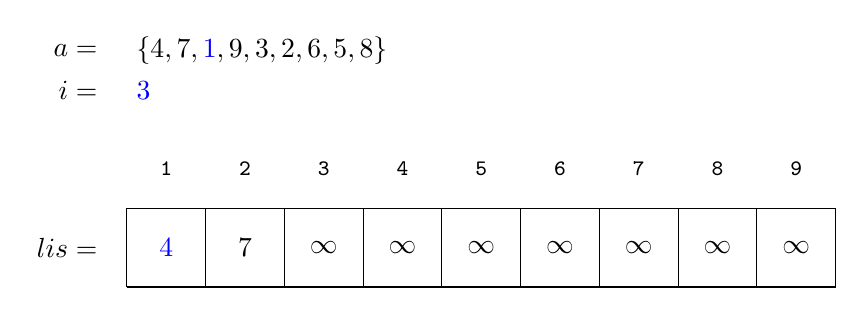
\begin{tikzpicture}

        \node[anchor=east] at (0.75, 4) { $a = $ };
        \node[anchor=west] at (1, 4) { $\{ \textcolor{black}{4}, \textcolor{black}{7}, \textcolor{blue}{1}, 9, 3, 2, 6, 5, 8 \}$ };
        \node[anchor=east] at (0.75, 3.5) { $i = $ };
        \node[anchor=west] at (1, 3.5) { $\textcolor{blue}{3}$ };

        \node[anchor=east] at (0.75, 1.5) { $lis = $ };
        \draw (1, 1) grid (10, 2);

        \foreach \x in {1, ..., 9}
            \node at (\x + 0.5, 2.5) { \footnotesize \textbf{\texttt{\x}} };

        \node at (1.5, 1.5) { \textcolor{blue}{$4$} };
        \node at (2.5, 1.5) { \textcolor{black}{$7$} };
        \node at (3.5, 1.5) { $\infty$ };
        \node at (4.5, 1.5) { $\infty$ };
        \node at (5.5, 1.5) { $\infty$ };
        \node at (6.5, 1.5) { $\infty$ };
        \node at (7.5, 1.5) { $\infty$ };
        \node at (8.5, 1.5) { $\infty$ };
        \node at (9.5, 1.5) { $\infty$ };
 
        \end{tikzpicture}
    \end{figure}

\end{frame}

\begin{frame}[fragile]{Visualização do algoritmo linearítmico para a LIS}

    \begin{figure}[h]
        \centering
        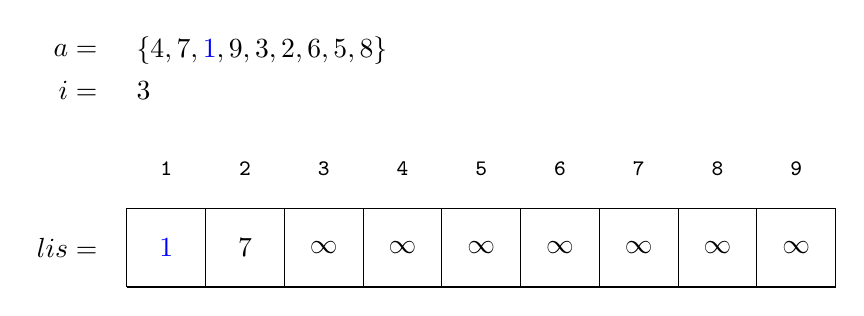
\begin{tikzpicture}

        \node[anchor=east] at (0.75, 4) { $a = $ };
        \node[anchor=west] at (1, 4) { $\{ \textcolor{black}{4}, \textcolor{black}{7}, \textcolor{blue}{1}, 9, 3, 2, 6, 5, 8 \}$ };
        \node[anchor=east] at (0.75, 3.5) { $i = $ };
        \node[anchor=west] at (1, 3.5) { $\textcolor{black}{3}$ };

        \node[anchor=east] at (0.75, 1.5) { $lis = $ };
        \draw (1, 1) grid (10, 2);

        \foreach \x in {1, ..., 9}
            \node at (\x + 0.5, 2.5) { \footnotesize \textbf{\texttt{\x}} };

        \node at (1.5, 1.5) { \textcolor{blue}{$1$} };
        \node at (2.5, 1.5) { \textcolor{black}{$7$} };
        \node at (3.5, 1.5) { $\infty$ };
        \node at (4.5, 1.5) { $\infty$ };
        \node at (5.5, 1.5) { $\infty$ };
        \node at (6.5, 1.5) { $\infty$ };
        \node at (7.5, 1.5) { $\infty$ };
        \node at (8.5, 1.5) { $\infty$ };
        \node at (9.5, 1.5) { $\infty$ };
 
        \end{tikzpicture}
    \end{figure}

\end{frame}

\begin{frame}[fragile]{Visualização do algoritmo linearítmico para a LIS}

    \begin{figure}[h]
        \centering
        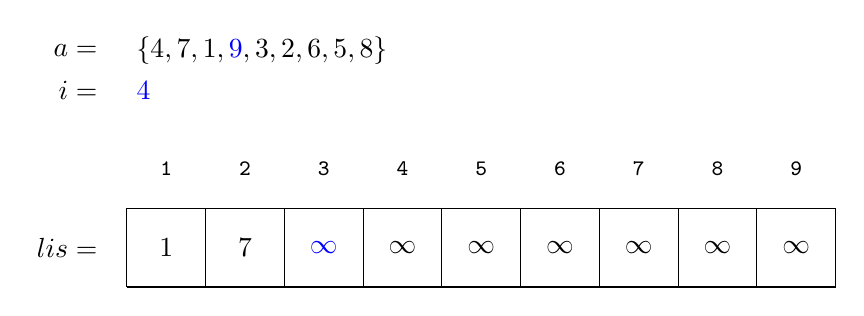
\begin{tikzpicture}

        \node[anchor=east] at (0.75, 4) { $a = $ };
        \node[anchor=west] at (1, 4) { $\{ \textcolor{black}{4}, \textcolor{black}{7}, \textcolor{black}{1}, \textcolor{blue}{9}, 3, 2, 6, 5, 8 \}$ };
        \node[anchor=east] at (0.75, 3.5) { $i = $ };
        \node[anchor=west] at (1, 3.5) { $\textcolor{blue}{4}$ };

        \node[anchor=east] at (0.75, 1.5) { $lis = $ };
        \draw (1, 1) grid (10, 2);

        \foreach \x in {1, ..., 9}
            \node at (\x + 0.5, 2.5) { \footnotesize \textbf{\texttt{\x}} };

        \node at (1.5, 1.5) { \textcolor{black}{$1$} };
        \node at (2.5, 1.5) { \textcolor{black}{$7$} };
        \node at (3.5, 1.5) { \textcolor{blue}{$\infty$} };
        \node at (4.5, 1.5) { $\infty$ };
        \node at (5.5, 1.5) { $\infty$ };
        \node at (6.5, 1.5) { $\infty$ };
        \node at (7.5, 1.5) { $\infty$ };
        \node at (8.5, 1.5) { $\infty$ };
        \node at (9.5, 1.5) { $\infty$ };
 
        \end{tikzpicture}
    \end{figure}

\end{frame}

\begin{frame}[fragile]{Visualização do algoritmo linearítmico para a LIS}

    \begin{figure}[h]
        \centering
        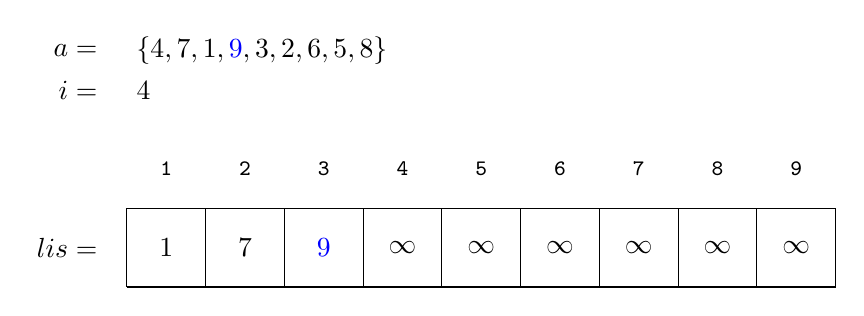
\begin{tikzpicture}

        \node[anchor=east] at (0.75, 4) { $a = $ };
        \node[anchor=west] at (1, 4) { $\{ \textcolor{black}{4}, \textcolor{black}{7}, \textcolor{black}{1}, \textcolor{blue}{9}, 3, 2, 6, 5, 8 \}$ };
        \node[anchor=east] at (0.75, 3.5) { $i = $ };
        \node[anchor=west] at (1, 3.5) { $\textcolor{black}{4}$ };

        \node[anchor=east] at (0.75, 1.5) { $lis = $ };
        \draw (1, 1) grid (10, 2);

        \foreach \x in {1, ..., 9}
            \node at (\x + 0.5, 2.5) { \footnotesize \textbf{\texttt{\x}} };

        \node at (1.5, 1.5) { \textcolor{black}{$1$} };
        \node at (2.5, 1.5) { \textcolor{black}{$7$} };
        \node at (3.5, 1.5) { \textcolor{blue}{$9$} };
        \node at (4.5, 1.5) { $\infty$ };
        \node at (5.5, 1.5) { $\infty$ };
        \node at (6.5, 1.5) { $\infty$ };
        \node at (7.5, 1.5) { $\infty$ };
        \node at (8.5, 1.5) { $\infty$ };
        \node at (9.5, 1.5) { $\infty$ };
 
        \end{tikzpicture}
    \end{figure}

\end{frame}

\begin{frame}[fragile]{Visualização do algoritmo linearítmico para a LIS}

    \begin{figure}[h]
        \centering
        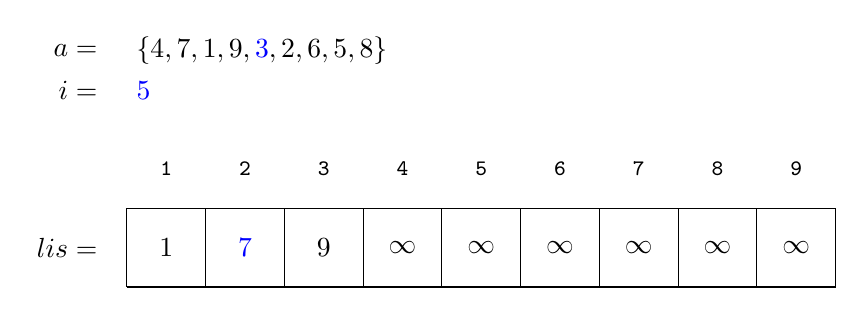
\begin{tikzpicture}

        \node[anchor=east] at (0.75, 4) { $a = $ };
        \node[anchor=west] at (1, 4) { $\{ \textcolor{black}{4}, \textcolor{black}{7}, \textcolor{black}{1}, \textcolor{black}{9}, \textcolor{blue}{3}, 2, 6, 5, 8 \}$ };
        \node[anchor=east] at (0.75, 3.5) { $i = $ };
        \node[anchor=west] at (1, 3.5) { $\textcolor{blue}{5}$ };

        \node[anchor=east] at (0.75, 1.5) { $lis = $ };
        \draw (1, 1) grid (10, 2);

        \foreach \x in {1, ..., 9}
            \node at (\x + 0.5, 2.5) { \footnotesize \textbf{\texttt{\x}} };

        \node at (1.5, 1.5) { \textcolor{black}{$1$} };
        \node at (2.5, 1.5) { \textcolor{blue}{$7$} };
        \node at (3.5, 1.5) { \textcolor{black}{$9$} };
        \node at (4.5, 1.5) { $\infty$ };
        \node at (5.5, 1.5) { $\infty$ };
        \node at (6.5, 1.5) { $\infty$ };
        \node at (7.5, 1.5) { $\infty$ };
        \node at (8.5, 1.5) { $\infty$ };
        \node at (9.5, 1.5) { $\infty$ };
 
        \end{tikzpicture}
    \end{figure}

\end{frame}

\begin{frame}[fragile]{Visualização do algoritmo linearítmico para a LIS}

    \begin{figure}[h]
        \centering
        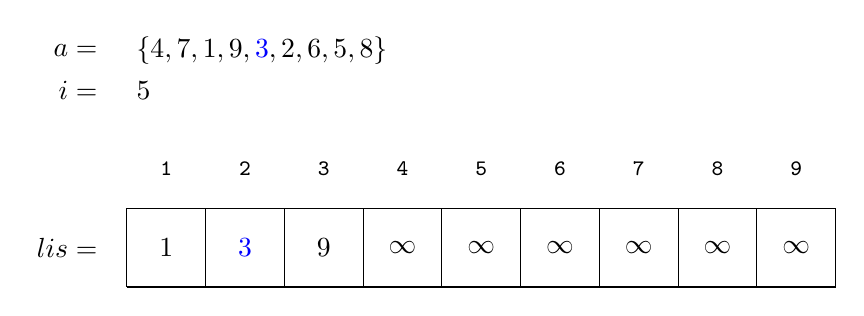
\begin{tikzpicture}

        \node[anchor=east] at (0.75, 4) { $a = $ };
        \node[anchor=west] at (1, 4) { $\{ \textcolor{black}{4}, \textcolor{black}{7}, \textcolor{black}{1}, \textcolor{black}{9}, \textcolor{blue}{3}, 2, 6, 5, 8 \}$ };
        \node[anchor=east] at (0.75, 3.5) { $i = $ };
        \node[anchor=west] at (1, 3.5) { $\textcolor{black}{5}$ };

        \node[anchor=east] at (0.75, 1.5) { $lis = $ };
        \draw (1, 1) grid (10, 2);

        \foreach \x in {1, ..., 9}
            \node at (\x + 0.5, 2.5) { \footnotesize \textbf{\texttt{\x}} };

        \node at (1.5, 1.5) { \textcolor{black}{$1$} };
        \node at (2.5, 1.5) { \textcolor{blue}{$3$} };
        \node at (3.5, 1.5) { \textcolor{black}{$9$} };
        \node at (4.5, 1.5) { $\infty$ };
        \node at (5.5, 1.5) { $\infty$ };
        \node at (6.5, 1.5) { $\infty$ };
        \node at (7.5, 1.5) { $\infty$ };
        \node at (8.5, 1.5) { $\infty$ };
        \node at (9.5, 1.5) { $\infty$ };
 
        \end{tikzpicture}
    \end{figure}

\end{frame}

\begin{frame}[fragile]{Visualização do algoritmo linearítmico para a LIS}

    \begin{figure}[h]
        \centering
        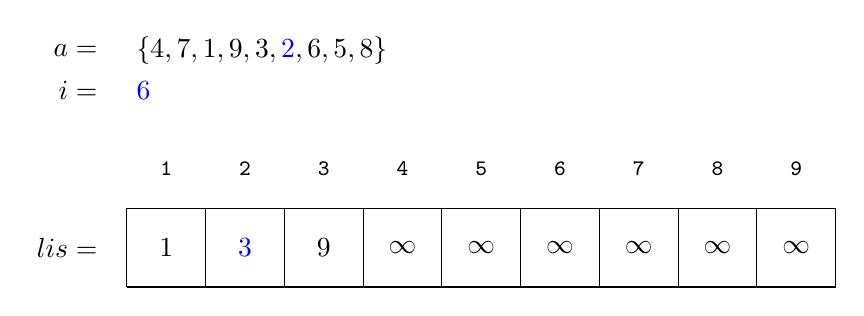
\begin{tikzpicture}

        \node[anchor=east] at (0.75, 4) { $a = $ };
        \node[anchor=west] at (1, 4) { $\{ \textcolor{black}{4}, \textcolor{black}{7}, \textcolor{black}{1}, \textcolor{black}{9}, \textcolor{black}{3}, \textcolor{blue}{2}, 6, 5, 8 \}$ };
        \node[anchor=east] at (0.75, 3.5) { $i = $ };
        \node[anchor=west] at (1, 3.5) { $\textcolor{blue}{6}$ };

        \node[anchor=east] at (0.75, 1.5) { $lis = $ };
        \draw (1, 1) grid (10, 2);

        \foreach \x in {1, ..., 9}
            \node at (\x + 0.5, 2.5) { \footnotesize \textbf{\texttt{\x}} };

        \node at (1.5, 1.5) { \textcolor{black}{$1$} };
        \node at (2.5, 1.5) { \textcolor{blue}{$3$} };
        \node at (3.5, 1.5) { \textcolor{black}{$9$} };
        \node at (4.5, 1.5) { $\infty$ };
        \node at (5.5, 1.5) { $\infty$ };
        \node at (6.5, 1.5) { $\infty$ };
        \node at (7.5, 1.5) { $\infty$ };
        \node at (8.5, 1.5) { $\infty$ };
        \node at (9.5, 1.5) { $\infty$ };
 
        \end{tikzpicture}
    \end{figure}

\end{frame}

\begin{frame}[fragile]{Visualização do algoritmo linearítmico para a LIS}

    \begin{figure}[h]
        \centering
        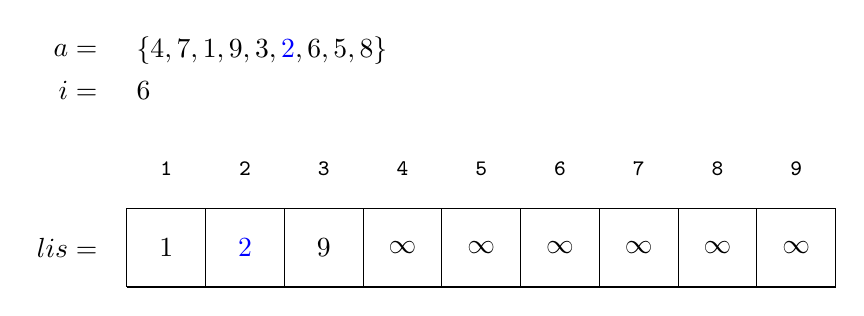
\begin{tikzpicture}

        \node[anchor=east] at (0.75, 4) { $a = $ };
        \node[anchor=west] at (1, 4) { $\{ \textcolor{black}{4}, \textcolor{black}{7}, \textcolor{black}{1}, \textcolor{black}{9}, \textcolor{black}{3}, \textcolor{blue}{2}, 6, 5, 8 \}$ };
        \node[anchor=east] at (0.75, 3.5) { $i = $ };
        \node[anchor=west] at (1, 3.5) { $\textcolor{black}{6}$ };

        \node[anchor=east] at (0.75, 1.5) { $lis = $ };
        \draw (1, 1) grid (10, 2);

        \foreach \x in {1, ..., 9}
            \node at (\x + 0.5, 2.5) { \footnotesize \textbf{\texttt{\x}} };

        \node at (1.5, 1.5) { \textcolor{black}{$1$} };
        \node at (2.5, 1.5) { \textcolor{blue}{$2$} };
        \node at (3.5, 1.5) { \textcolor{black}{$9$} };
        \node at (4.5, 1.5) { $\infty$ };
        \node at (5.5, 1.5) { $\infty$ };
        \node at (6.5, 1.5) { $\infty$ };
        \node at (7.5, 1.5) { $\infty$ };
        \node at (8.5, 1.5) { $\infty$ };
        \node at (9.5, 1.5) { $\infty$ };
 
        \end{tikzpicture}
    \end{figure}

\end{frame}

\begin{frame}[fragile]{Visualização do algoritmo linearítmico para a LIS}

    \begin{figure}[h]
        \centering
        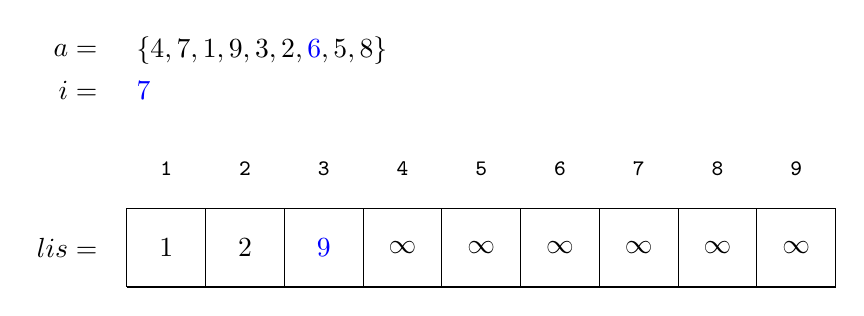
\begin{tikzpicture}

        \node[anchor=east] at (0.75, 4) { $a = $ };
        \node[anchor=west] at (1, 4) { $\{ \textcolor{black}{4}, \textcolor{black}{7}, \textcolor{black}{1}, \textcolor{black}{9}, \textcolor{black}{3}, \textcolor{black}{2}, \textcolor{blue}{6}, 5, 8 \}$ };
        \node[anchor=east] at (0.75, 3.5) { $i = $ };
        \node[anchor=west] at (1, 3.5) { $\textcolor{blue}{7}$ };

        \node[anchor=east] at (0.75, 1.5) { $lis = $ };
        \draw (1, 1) grid (10, 2);

        \foreach \x in {1, ..., 9}
            \node at (\x + 0.5, 2.5) { \footnotesize \textbf{\texttt{\x}} };

        \node at (1.5, 1.5) { \textcolor{black}{$1$} };
        \node at (2.5, 1.5) { \textcolor{black}{$2$} };
        \node at (3.5, 1.5) { \textcolor{blue}{$9$} };
        \node at (4.5, 1.5) { $\infty$ };
        \node at (5.5, 1.5) { $\infty$ };
        \node at (6.5, 1.5) { $\infty$ };
        \node at (7.5, 1.5) { $\infty$ };
        \node at (8.5, 1.5) { $\infty$ };
        \node at (9.5, 1.5) { $\infty$ };
 
        \end{tikzpicture}
    \end{figure}

\end{frame}

\begin{frame}[fragile]{Visualização do algoritmo linearítmico para a LIS}

    \begin{figure}[h]
        \centering
        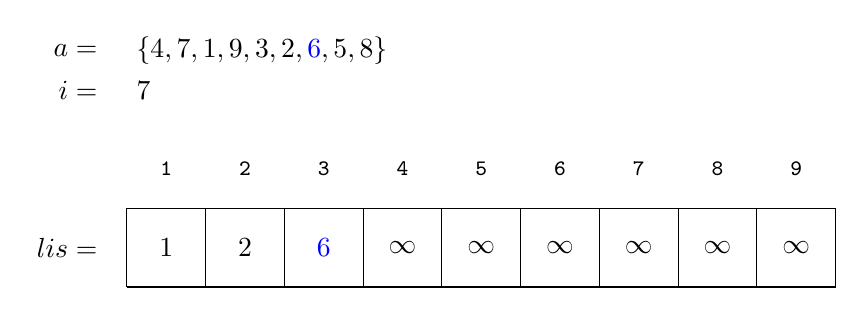
\begin{tikzpicture}

        \node[anchor=east] at (0.75, 4) { $a = $ };
        \node[anchor=west] at (1, 4) { $\{ \textcolor{black}{4}, \textcolor{black}{7}, \textcolor{black}{1}, \textcolor{black}{9}, \textcolor{black}{3}, \textcolor{black}{2}, \textcolor{blue}{6}, 5, 8 \}$ };
        \node[anchor=east] at (0.75, 3.5) { $i = $ };
        \node[anchor=west] at (1, 3.5) { $\textcolor{black}{7}$ };

        \node[anchor=east] at (0.75, 1.5) { $lis = $ };
        \draw (1, 1) grid (10, 2);

        \foreach \x in {1, ..., 9}
            \node at (\x + 0.5, 2.5) { \footnotesize \textbf{\texttt{\x}} };

        \node at (1.5, 1.5) { \textcolor{black}{$1$} };
        \node at (2.5, 1.5) { \textcolor{black}{$2$} };
        \node at (3.5, 1.5) { \textcolor{blue}{$6$} };
        \node at (4.5, 1.5) { $\infty$ };
        \node at (5.5, 1.5) { $\infty$ };
        \node at (6.5, 1.5) { $\infty$ };
        \node at (7.5, 1.5) { $\infty$ };
        \node at (8.5, 1.5) { $\infty$ };
        \node at (9.5, 1.5) { $\infty$ };
 
        \end{tikzpicture}
    \end{figure}

\end{frame}

\begin{frame}[fragile]{Visualização do algoritmo linearítmico para a LIS}

    \begin{figure}[h]
        \centering
        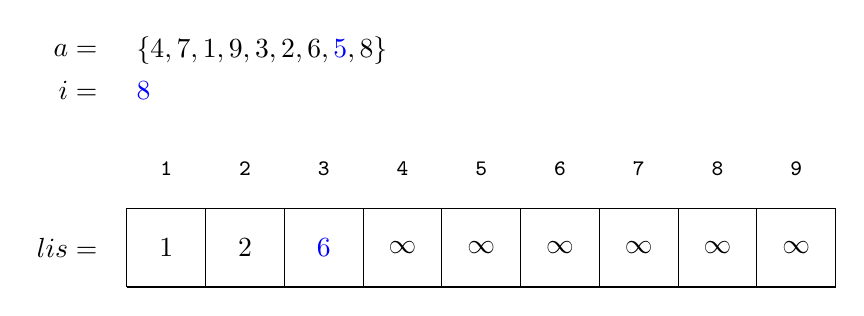
\begin{tikzpicture}

        \node[anchor=east] at (0.75, 4) { $a = $ };
        \node[anchor=west] at (1, 4) { $\{ \textcolor{black}{4}, \textcolor{black}{7}, \textcolor{black}{1}, \textcolor{black}{9}, \textcolor{black}{3}, \textcolor{black}{2}, \textcolor{black}{6}, \textcolor{blue}{5}, 8 \}$ };
        \node[anchor=east] at (0.75, 3.5) { $i = $ };
        \node[anchor=west] at (1, 3.5) { $\textcolor{blue}{8}$ };

        \node[anchor=east] at (0.75, 1.5) { $lis = $ };
        \draw (1, 1) grid (10, 2);

        \foreach \x in {1, ..., 9}
            \node at (\x + 0.5, 2.5) { \footnotesize \textbf{\texttt{\x}} };

        \node at (1.5, 1.5) { \textcolor{black}{$1$} };
        \node at (2.5, 1.5) { \textcolor{black}{$2$} };
        \node at (3.5, 1.5) { \textcolor{blue}{$6$} };
        \node at (4.5, 1.5) { $\infty$ };
        \node at (5.5, 1.5) { $\infty$ };
        \node at (6.5, 1.5) { $\infty$ };
        \node at (7.5, 1.5) { $\infty$ };
        \node at (8.5, 1.5) { $\infty$ };
        \node at (9.5, 1.5) { $\infty$ };
 
        \end{tikzpicture}
    \end{figure}

\end{frame}

\begin{frame}[fragile]{Visualização do algoritmo linearítmico para a LIS}

    \begin{figure}[h]
        \centering
        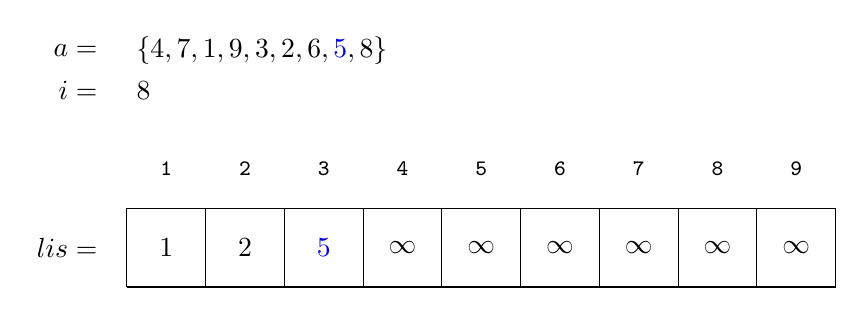
\begin{tikzpicture}

        \node[anchor=east] at (0.75, 4) { $a = $ };
        \node[anchor=west] at (1, 4) { $\{ \textcolor{black}{4}, \textcolor{black}{7}, \textcolor{black}{1}, \textcolor{black}{9}, \textcolor{black}{3}, \textcolor{black}{2}, \textcolor{black}{6}, \textcolor{blue}{5}, 8 \}$ };
        \node[anchor=east] at (0.75, 3.5) { $i = $ };
        \node[anchor=west] at (1, 3.5) { $\textcolor{black}{8}$ };

        \node[anchor=east] at (0.75, 1.5) { $lis = $ };
        \draw (1, 1) grid (10, 2);

        \foreach \x in {1, ..., 9}
            \node at (\x + 0.5, 2.5) { \footnotesize \textbf{\texttt{\x}} };

        \node at (1.5, 1.5) { \textcolor{black}{$1$} };
        \node at (2.5, 1.5) { \textcolor{black}{$2$} };
        \node at (3.5, 1.5) { \textcolor{blue}{$5$} };
        \node at (4.5, 1.5) { $\infty$ };
        \node at (5.5, 1.5) { $\infty$ };
        \node at (6.5, 1.5) { $\infty$ };
        \node at (7.5, 1.5) { $\infty$ };
        \node at (8.5, 1.5) { $\infty$ };
        \node at (9.5, 1.5) { $\infty$ };
 
        \end{tikzpicture}
    \end{figure}

\end{frame}

\begin{frame}[fragile]{Visualização do algoritmo linearítmico para a LIS}

    \begin{figure}[h]
        \centering
        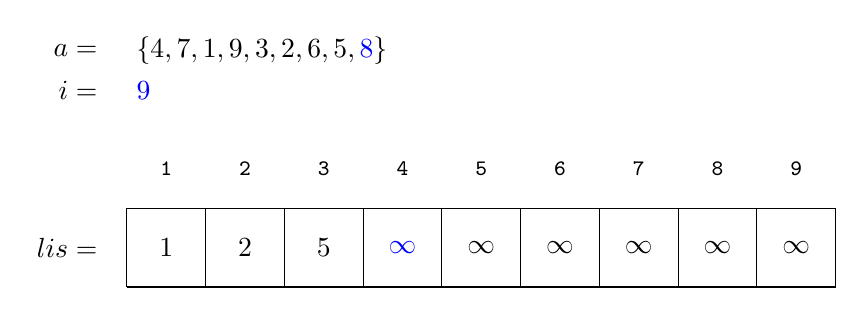
\begin{tikzpicture}

        \node[anchor=east] at (0.75, 4) { $a = $ };
        \node[anchor=west] at (1, 4) { $\{ \textcolor{black}{4}, \textcolor{black}{7}, \textcolor{black}{1}, \textcolor{black}{9}, \textcolor{black}{3}, \textcolor{black}{2}, \textcolor{black}{6}, \textcolor{black}{5}, \textcolor{blue}{8} \}$ };
        \node[anchor=east] at (0.75, 3.5) { $i = $ };
        \node[anchor=west] at (1, 3.5) { $\textcolor{blue}{9}$ };

        \node[anchor=east] at (0.75, 1.5) { $lis = $ };
        \draw (1, 1) grid (10, 2);

        \foreach \x in {1, ..., 9}
            \node at (\x + 0.5, 2.5) { \footnotesize \textbf{\texttt{\x}} };

        \node at (1.5, 1.5) { \textcolor{black}{$1$} };
        \node at (2.5, 1.5) { \textcolor{black}{$2$} };
        \node at (3.5, 1.5) { \textcolor{black}{$5$} };
        \node at (4.5, 1.5) { \textcolor{blue}{$\infty$} };
        \node at (5.5, 1.5) { $\infty$ };
        \node at (6.5, 1.5) { $\infty$ };
        \node at (7.5, 1.5) { $\infty$ };
        \node at (8.5, 1.5) { $\infty$ };
        \node at (9.5, 1.5) { $\infty$ };
 
        \end{tikzpicture}
    \end{figure}

\end{frame}

\begin{frame}[fragile]{Visualização do algoritmo linearítmico para a LIS}

    \begin{figure}[h]
        \centering
        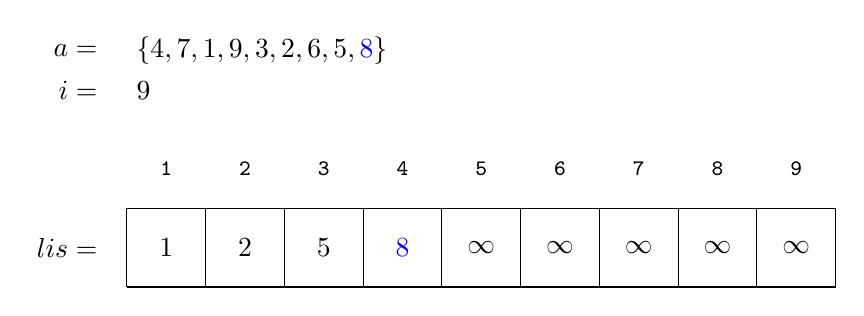
\begin{tikzpicture}

        \node[anchor=east] at (0.75, 4) { $a = $ };
        \node[anchor=west] at (1, 4) { $\{ \textcolor{black}{4}, \textcolor{black}{7}, \textcolor{black}{1}, \textcolor{black}{9}, \textcolor{black}{3}, \textcolor{black}{2}, \textcolor{black}{6}, \textcolor{black}{5}, \textcolor{blue}{8} \}$ };
        \node[anchor=east] at (0.75, 3.5) { $i = $ };
        \node[anchor=west] at (1, 3.5) { $\textcolor{black}{9}$ };

        \node[anchor=east] at (0.75, 1.5) { $lis = $ };
        \draw (1, 1) grid (10, 2);

        \foreach \x in {1, ..., 9}
            \node at (\x + 0.5, 2.5) { \footnotesize \textbf{\texttt{\x}} };

        \node at (1.5, 1.5) { \textcolor{black}{$1$} };
        \node at (2.5, 1.5) { \textcolor{black}{$2$} };
        \node at (3.5, 1.5) { \textcolor{black}{$5$} };
        \node at (4.5, 1.5) { \textcolor{blue}{$8$} };
        \node at (5.5, 1.5) { $\infty$ };
        \node at (6.5, 1.5) { $\infty$ };
        \node at (7.5, 1.5) { $\infty$ };
        \node at (8.5, 1.5) { $\infty$ };
        \node at (9.5, 1.5) { $\infty$ };
 
        \end{tikzpicture}
    \end{figure}

\end{frame}


\begin{frame}[fragile]{Implementação da LCS como LIS em C++}
    \inputsnippet{cpp}{5}{21}{codes/lis.cpp}
\end{frame}

\begin{frame}[fragile]{Implementação da LCS como LIS em C++}
    \inputsnippet{cpp}{23}{41}{codes/lis.cpp}
\end{frame}
